\chapter{Remarks about our study}
In this chapter we are going to describe in detail the specifications of the simulations we are going to work with, as well as the method for determining the halo shapes. This shapter is mainly to thoroughly explain how are we going to do everything that we are going to do.\\

\section{The Auriga simulations}
Cosmological simulations are restricted to modeling DM as a non collisional fluid and gas as an Eulerian(?) collisional fluid. Efficiently solving these systems of non-linear equations is an intrincate puzzle and it is still an open and improving field of research. 
Difficulties in the numerical modelling of these fluids arise from the wide range of values that quantities take in the context of cosmological objects, which can expand in several orders of magnitude, are no much different than actual field discontinuities which are very difficult to treat in a numerical way.\\

It is clear that this simulations are limited to some resolution depending on the current power of computing super-clusters. This resolution is variable between simulations and is adjustable to the specific objective of the research. However, this resolution is by no means sufficient to simulate specific termic processes dominated by quantum or particle physics. However, specific details which are consequence of this non-modelable physics, are needed to accurately model cosmological structures. This is why energy and mass feedback processes such as supernovae (SN) explosions, black hole (BH) accretion and radiation, are usually reduced to some simplification dependent on some free parameters. A decade ago, thee feedback processes were not as well understood nor well modelled as they are today. For this reason, and the advances on technology, it has been possible only until recently the simulation of galactic-sized objects like our MW tracking the evolution of normal matter alongside with DM.\\


State all the important specs of the Auriga simulations. On the first paragraph.\\

Talk about the different degrees of realism in this simulation> DM, MHD, resolution levels. State the importance of these aspects for the soundness (look better word) of the studies.\\

\begin{figure}[!ht]
    \centering
    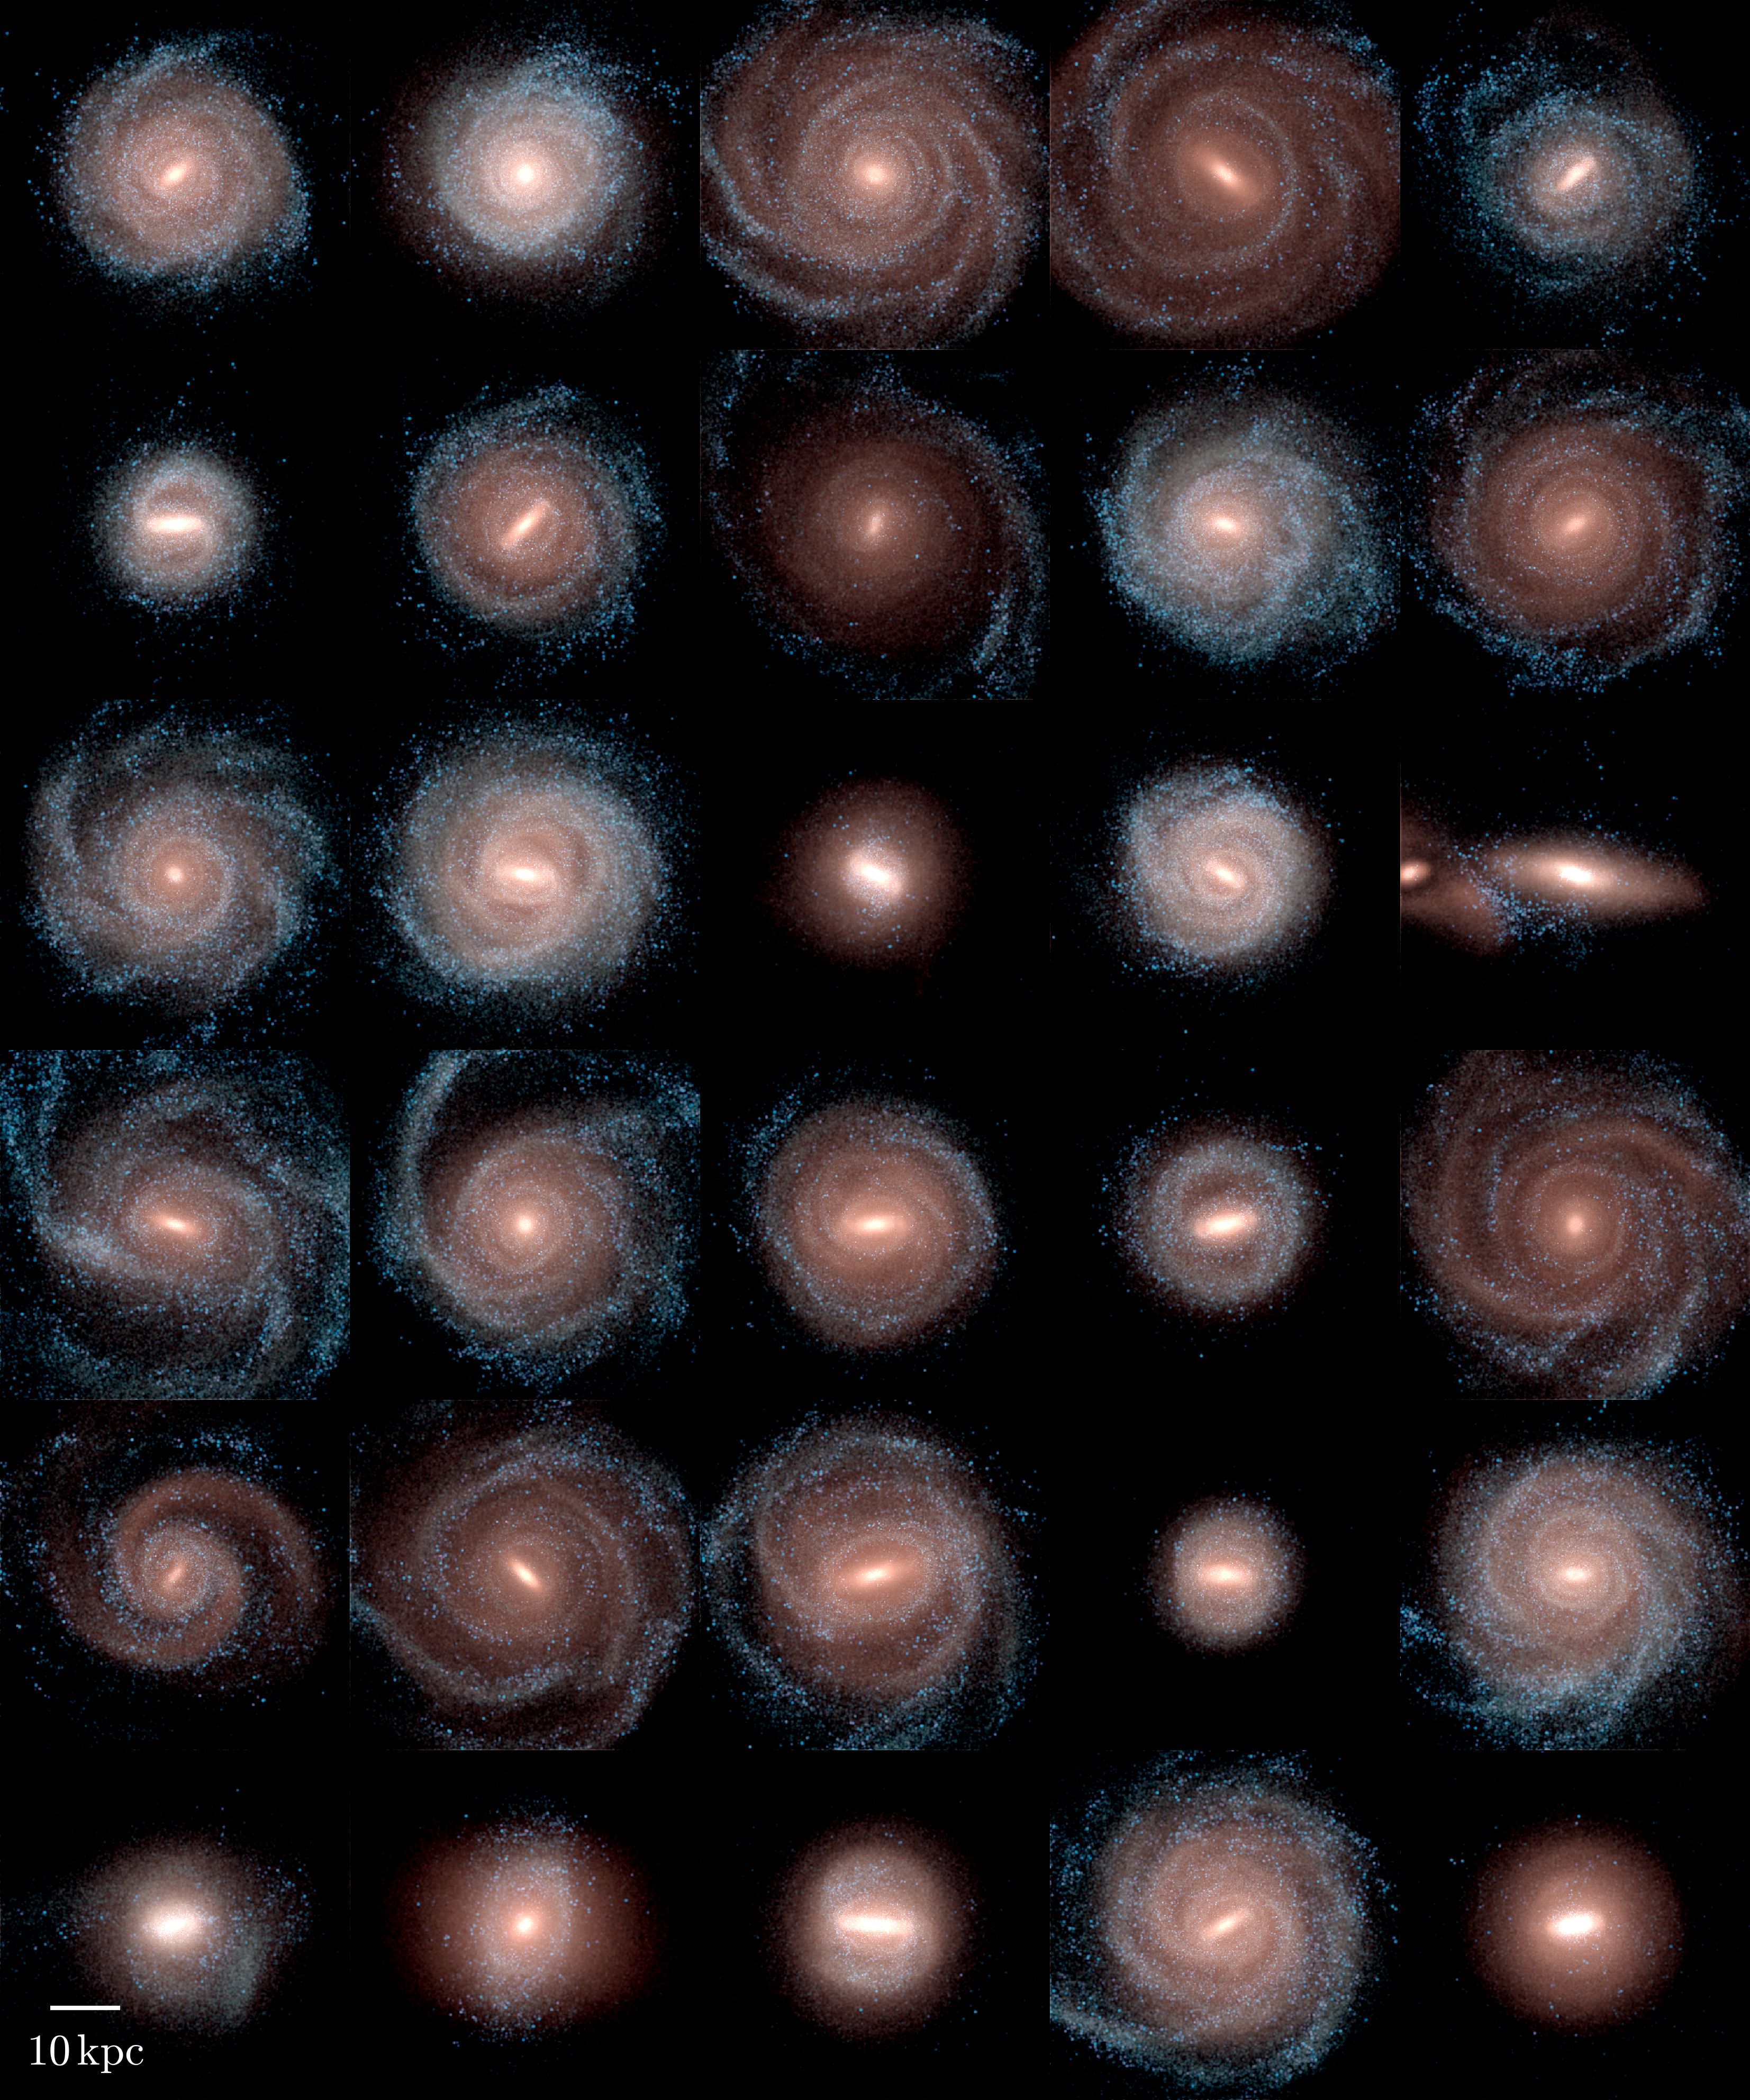
\includegraphics[width=0.8\textwidth]{./pics/Auriga.png}
    \caption{Set of 30 MW-like simulations, taken from http://auriga.h-its.org/}
    \label{fig:auriga}
\end{figure}

\section{Determining the halo shape}
Start saying that there is no unique method for determining the shape at a specific radius. In general this process is not trivial and there are many different(in theory) approaches which produce esentially the same results \cite{Vera-Ciro2010}. Mention that we are going to use method by Allgood et al 2006 \cite{AllGood2006} following the steps by Vera-Ciro2010.\\

The method starts with particles enclosed within a sphere, we calculate the reduced inertia tensor:

\begin{equation}
I_{ij} = \sum_k \frac{x_k^{(i)}x_k^{(j)}}{d^2_k},
\label{eq:inertia}
\end{equation}

that is not sufficient, which is why we recalculate until we achieve convergence. Present this recalculation explicitly with a scale transformation which intuitively means that our ellipse is becoming a sphere under that transformation which at the end is fully consistent (find better words).

\begin{align}
(x,y,z) &\rightarrow (x,y/q,z/s) \label{eq:scale}\\
q &=  b/a \nonumber \\
s &= c/a \nonumber ,
\end{align}

Specify that with this process we obtain both the radial profile and the historical shape by simply applying this method at different radii and redshifts.
